%!TEX root = project.tex

\chapter{System Evaluation}
\section{Testing}

\begin{itemize}
\item Prove that your software is robust. How? Testing etc. 
\item Use performance benchmarks (space and time) if algorithmic.
\item Measure the outcomes / outputs of your system / software against the objectives from the Introduction.
\item Highlight any limitations or opportunities in your approach or technologies used.
\end{itemize}


\section{Drawbacks and Limitations}
Testing proved difficult on a standard PC. Unity 3d is a large and powerful piece of software that requires a lot of resources to run. This resulted in slow performance when testing for some members of the team. When tested on a standard laptop we found the game was extremely taxing on the GPU, 86 - 95\% output at times.
\newline

As a result the game would work fine from the login process to the procedural track generation but would sometimes result in the game character not begin able to move forward. Alternatively when run on custom built gaming PCs, which two members of the group have, they experienced no problems at all.
\newline

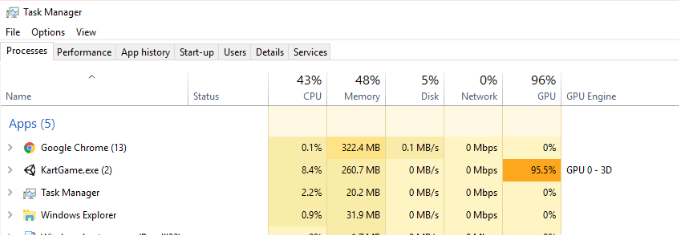
\includegraphics[width=1\columnwidth]{img/output.PNG}
\newline
 
Another slight drawback was working with MongoDB as it was sometimes troublesome due to a lot of the java syntax for mongo being deprecated. A maven project approach might have been a better idea as there are more resources available with regards to working with mongo using java. 
\newline

The AWS virtual machine we used served its purpose as a free option but the initial set up of the power of the machine was basic. We found out, throughout the development process, that we needed to restrict the amount of software installations on the VM. This was brought to our attention when the VMs performance had become extremely sluggish and sometimes unresponsive. As a result we decided to discuss any future software installations unless it was vital to the project. The removal of the eclipse IDE was a necessary step once the login process was up and running. This helped free up some space and memory for other resources that needed to be constantly active and running. In future, the implementation of a dedicated server to run the data bases might be a better option.

\section{Outcomes}
The project goals, as laid out in the introduction, was a success to a point. The processes involved in allowing a player to login works very well. The database and program running this process has been running since the start of the project and has never given us any difficulty since being implemented.
\newline

The hosting and joining system also works very well. The data that is required when sending and receiving to and from the databases does so very efficiently.    





